%
%-----------------------------------
\section{Dysprosium}
\label{sec:dysprosium}
%-----------------------------------
%

\begin{table}[ht!]
    \centering
    \begin{tabular}{|c|c|c|}
        \hline
        \textbf{Symbol} & \textbf{Quantity} & \textbf{Value} \\ \hline
        $ T_D $ & Doppler temperature & $ 3.26\ \mu K $ \\
        $ \Gamma $ & Natural Linewidth & $ 2\pi \times 136\ kHz $ \\
        $ \lambda $ & Resonant wavelength & $ 626\ nm $ \\
        $ J_{gnd} $ & Ground state angular momentum & $ 8 $ \\
        $ g_{gnd} $ & Ground state Landè factor & $ 1.24 $ \\
        $ g_{exc} $ & Excited state Landè factor & $ 1.29 $ \\
        $ m $ & Mass & $ 164\ u $ \\
        $ Z $ & Atomic number & $ 66 $ \\
        \hline
    \end{tabular}
    \caption{$ {}^{164}Dy $ features and transition information.}
    \label{tab:164Dy}
\end{table}

\begin{table}[ht!]
    \centering
    \begin{tabular}{|c|c|c|}
        \hline
        \textbf{Symbol} & \textbf{Quantity} & \textbf{Value} \\ \hline
        $ w $ & Waist & $ 2.0\ cm $ \\
        $ s_0 $ & Saturation parameter & $ 0.65 $ \\
        \hline
    \end{tabular}
    \caption{Laser setup features}
    \label{tab:lasers-setup}
\end{table}

\begin{table}[ht!]
    \centering
    \begin{tabular}{|c|c|c|}
        \hline
        \textbf{Symbol} & \textbf{Quantity} & \textbf{Value} \\ \hline
        $ B_0 $ & Axial gradient & $ 1.71 G $ \\
        $ B $ & Magnetic Field & $ B_0(-\hat{x} + \hat{y}/2 + \hat{z} / 2) $ \\
        $ B_{bias} $ & Bias & $ (-0.094 \hat{z})\ G / cm $ \\
        \hline
    \end{tabular}
    \caption{Magnetic quadrupole field}
    \label{tab:magnetic-field}
\end{table}

%-----------------------------------
\subsection{Atomic cloud profile}
\label{sec:cloud-profile-dysprosium}
%-----------------------------------

\begin{figure}[!ht]
    \centering
    \caption{Simulated ${}^{164}Dy$ cloud profile}
    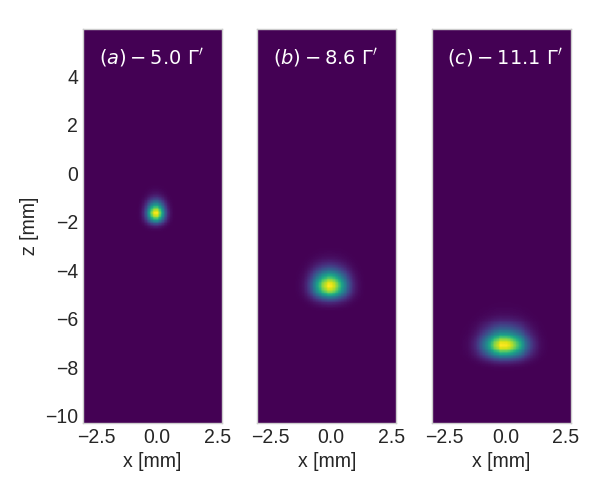
\includegraphics[width=0.7\textwidth]{USPSC-img/dy_dreon_cloud_profile.png}
    \vspace{5px}
    \legend{Simulated dysprosium cloud profile for three laser detunings: $ \delta = -5.0\Gamma' $ (a), $ \delta = -8.6\Gamma' $ (b), and $ \delta = -11.1\Gamma' $ (c), where $ \Gamma' = \Gamma \sqrt{1 + s_0} $ is the power-broadened linewidth. \\ Source: author}
    \label{fig:dy-atomic-cloud-profile}
\end{figure}

\begin{figure}[!ht]
    \centering
    \caption{Centre of mass of the ${}^{164}Dy$ nMOT}
    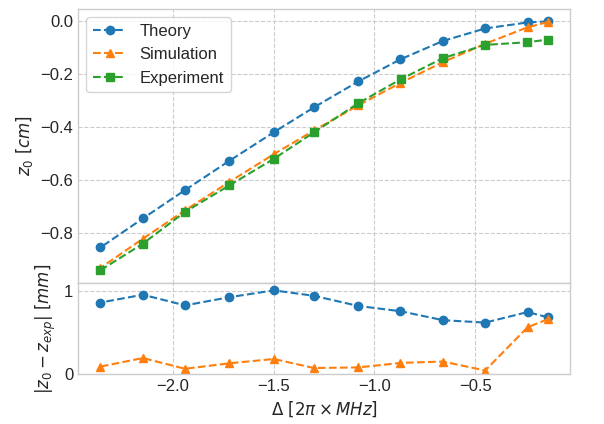
\includegraphics[width=0.7\textwidth]{USPSC-img/dy_centre_of_mass.png}
    \vspace{5px}
    \legend{centre of mass.\\ Source: author}
    \label{fig:dy-centre-of-mass}
\end{figure}

\begin{figure}[!ht]
    \centering
    \caption{Cloud size of the ${}^{164}Dy$ nMOT}
    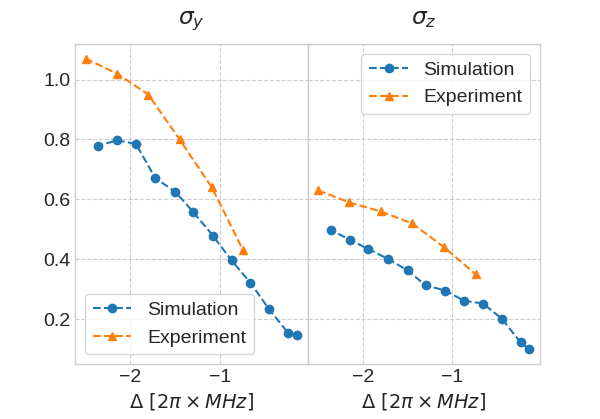
\includegraphics[width=0.7\textwidth]{USPSC-img/dy_cloud_size.png}
    \vspace{5px}
    \legend{cloud size.\\ Source: author}
    \label{fig:dy-cloud-size}
\end{figure}

\begin{figure}[!ht]
    \centering
    \caption{Cloud size ratio of the ${}^{164}Dy$ nMOT}
    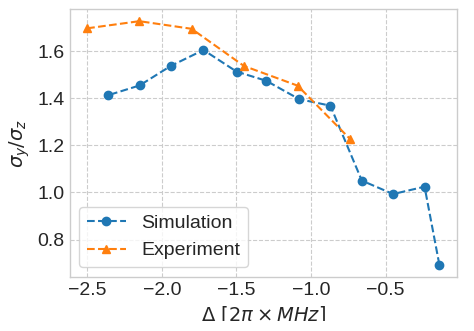
\includegraphics[width=0.55\textwidth]{USPSC-img/dy_cloud_size_ratio.png}
    \vspace{5px}
    \legend{cloud size ratio.\\ Source: author}
    \label{fig:dy-cloud-size-ratio}
\end{figure}

%-----------------------------------
\subsection{Temperature}
\label{temperature}
%-----------------------------------

\begin{figure}[!ht]
    \centering
    \caption{Temperature of the ${}^{164}Dy$ nMOT as a function of the laser detuning}
    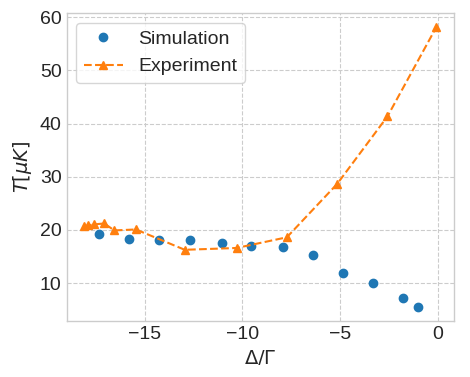
\includegraphics[width=0.6\textwidth]{USPSC-img/dy_temperature.png}
    \vspace{5px}
    \legend{temperature.\\ Source: author}
    \label{fig:dy-temperature}
\end{figure}
